%%%%%%%%%%%%%%%%%%%%%%%%%%%%%%%%%%%%%%%%%
% University Assignment Title Page 
% LaTeX Template
% Version 1.0 (27/12/12)
%
% This template has been downloaded from:
% http://www.LaTeXTemplates.com
%
% Original author:
% WikiBooks (http://en.wikibooks.org/wiki/LaTeX/Title Creation)
%
% License:
% CC BY-NC-SA 3.0 (http://creativecommons.org/licenses/by-nc-sa/3.0/)
% 
% Instructions for using this template:
% This title page is capable of being compiled as is. This is not useful for 
% including it in another document. To do this, you have two options: 
%
% 1) Copy/paste everything between \begin{document} and \end{document} 
% starting at \begin{titlepage} and paste this into another LaTeX file where you 
% want your title page.
% OR
% 2) Remove everything outside the \begin{titlepage} and \end{titlepage} and 
% move this file to the same directory as the LaTeX file you wish to add it to. 
% Then add \input{./title page_1.tex} to your LaTeX file where you want your
% title page.
%
%%%%%%%%%%%%%%%%%%%%%%%%%%%%%%%%%%%%%%%%%

%----------------------------------------------------------------------------------------
%	PACKAGES AND OTHER DOCUMENT CONFIGURATIONS
%----------------------------------------------------------------------------------------

\documentclass[12pt]{article}
\usepackage{graphicx}
\usepackage[utf8]{inputenc}  
\usepackage[T1]{fontenc} 
\usepackage[top=1cm,bottom=1cm,left=0.5cm,right=1.5cm,asymmetric]{geometry}
\usepackage{amsfonts}
\usepackage{graphicx}
\usepackage{algorithm}
\usepackage{algpseudocode}
\usepackage{amsmath, amssymb}
\usepackage{caption}
\usepackage{mathtools}
\usepackage{subcaption}
\usepackage{float}
\usepackage{subfig}
\usepackage{fancyhdr}
\pagestyle{fancy}
\renewcommand{\footrulewidth}{1pt}
\fancyhead[R]{\textit{Master MVA : Simulation based learning}}
\fancyfoot[L]{\textit{}}
%\usepackage{unicode-math}
%\setmathfont{XITS Math}
%\setmathfont[version=setB,StylisticSet=1]{XITS Math}
\usepackage{array,multirow,makecell}
\setcellgapes{1pt}
\makegapedcells
\newcolumntype{R}[1]{>{\raggedleft\arraybackslash }b{#1}}
\newcolumntype{L}[1]{>{\raggedright\arraybackslash }b{#1}}
\newcolumntype{C}[1]{>{\centering\arraybackslash }b{#1}}

\pagestyle{fancy}
\renewcommand{\footrulewidth}{1pt}
\fancyfoot[L]{\textit{}}
\newcommand{\cond}{(x_i|x_{\pi_i})}

%\usepackage{caption}
%\usepackage{subcaption}


%\usepackage{unicode-math}
%\setmathfont{XITS Math}
%\setmathfont[version=setB,StylisticSet=1]{XITS Math}


%\geometry{hmargin=1.5cm,vmargin=2cm}   

\geometry{hmargin=2.5cm,vmargin=2cm}   
\begin{document}
	
	\section*{Homework 4 (HW4 Part B)}
	\section*{Oussama Ennafii \& Sammy Khalife}
	\subsubsection*{25/02/2015}

\section*{Step 1}
~\\

1. The equality is trivial: we just have to set $\vartheta=\theta$.\\

To prove the inequality $$ Q_{\gamma}(\vartheta,\theta)\geq (f+g)(\vartheta)$$ we just need to prove that:

$$\forall \vartheta , \theta \in \Theta \quad f(\vartheta)\leq f(\theta)+<\nabla f(\theta),\vartheta-\theta>+\frac{1}{2\gamma}\vert\vert \vartheta-\theta\vert\vert^2$$

Set $ \vartheta , \theta \in \Theta$. Let's take $t \in [0,1]$, we define:

\begin{equation}
F(t) \triangleq f(\vartheta_t)-f(\theta)-<\nabla f(\theta),\vartheta_t-\theta>-\frac{1}{2\gamma}\vert\vert \vartheta_t-\theta\vert\vert^2
\end{equation}

where $\vartheta_t=t \vartheta+(1-t)\theta$. Since, $\frac{d}{dt}\vartheta_t=\vartheta-\theta$, $F$ is differentiable and:

\begin{eqnarray*}
	\frac{d}{dt}F(t)&=& <\nabla f(\vartheta), \vartheta-\theta> - <\nabla f(\theta), \vartheta-\theta>-\frac{1}{\gamma}\vert\vert \vartheta-\theta\vert\vert^2\\
						&=& <\nabla f(\vartheta)- \nabla f(\theta), \vartheta-\theta> -\frac{1}{\gamma}\vert\vert \vartheta-\theta\vert\vert^2\\
						&\leq& \vert\vert  \nabla f(\vartheta)- \nabla f(\theta)\vert \vert . \vert \vert \vartheta-\theta\vert \vert -\vert\vert \vartheta-\theta\vert\vert^2\\
						&\leq& (L-\frac{1}{\gamma})\vert\vert \vartheta-\theta\vert\vert^2\\
						&\leq& 0
\end{eqnarray*}

The first inequality is the result of Cauchy-Schwartz inequality while the second one is due to the Lipschitz nature of the gradient. The third inequality comes from the fact that $0<\gamma\leq \frac{1}{L}$.\\
This means that $F$ in decreasing in $[0,1]$, so: $F(0)\geq F(1)$:
$$F(0)=0$$
and :
$$F(1)=f(\vartheta)- f(\theta)-<\nabla f(\theta),\vartheta-\theta>-\frac{1}{2\gamma}\vert\vert \vartheta-\theta\vert\vert^2$$

2. Let $n \in \mathbb{N}$:

\begin{eqnarray*}
	(f+g)(\theta_{n})&=& Q_{\gamma_{n+1}}(\theta_{n},\theta_{n})\\
							&\geq& Q_{\gamma_{n+1}}(\theta_{n+1},\theta_{n})\\ 
							&\geq& (f+g)(\theta_{n+1})
\end{eqnarray*}
The first inequality is the result of the definition of $\theta_{n+1}$. The second one comes from the first question.\\

3. Set $ \vartheta , \theta \in \Theta$. we develop: 

\begin{eqnarray*}
	\frac{1}{2\gamma}\vert\vert \vartheta - \theta -\gamma \nabla f(\theta) \vert\vert^2&=&\frac{1}{2\gamma}\vert\vert \vartheta - \theta \vert \vert ^2 - <\vartheta - \theta ,\nabla f(\theta)>+\frac{\gamma}{2} \vert\vert \nabla f(\theta)\vert\vert^2
\end{eqnarray*}

This means that :

$$Q_{\gamma}(\vartheta,\theta)= g(\vartheta)+f(\theta)+ 	\frac{1}{2\gamma}\vert\vert \vartheta - \theta -\gamma \nabla f(\theta) \vert\vert^2-\frac{\gamma}{2} \vert\vert \nabla f(\theta)\vert\vert^2$$

4. Taking off the constants w.r.t to $\vartheta$, we get:

\begin{eqnarray*}
	\theta_{n+1}&=& \text{arg min}_{\vartheta \in \Theta} Q_{\gamma_{n+1}} (\vartheta,\theta_n)\\
						&=& \text{arg min}_{\vartheta \in \Theta} g(\vartheta)+\frac{1}{2\gamma_{n+1}}\vert\vert \vartheta - \theta_n -\gamma_{n+1} \nabla f(\theta_n) \vert\vert^2\\
						&=& \text{arg min}_{\vartheta \in \Theta} \sum_{i=1,\dots,d} \lambda \vert \vartheta_i \vert 
					 + \frac{1}{2\gamma_{n+1}}( \vartheta_i -( \theta_n)_i - \gamma_{n+1}( \nabla f(\theta_n))_i )^2
\end{eqnarray*}

So we can just minimize on each direction independently:

$$(\theta_{n+1})_i= \text{arg min}_{\vartheta_i} \lambda \vert \vartheta_i \vert+ \frac{1}{2\gamma_{n+1}}( \vartheta_i - ( \theta_n)_i -\gamma_{n+1}( \nabla f(\theta_n))_i )^2$$

We set : $u= \theta_n-\gamma_{n+1}\nabla f(\theta_n)$. We rewrite the last equation as:
$$(\theta_{n+1})_i= \text{arg min}_{\vartheta_i} \lambda \vert \vartheta_i \vert + \frac{1}{2 \gamma_{n+1}}( \vartheta_i - u_i)^2$$

So we consider the function:
$$L^{\gamma}_u(x)\triangleq \lambda \vert x \vert+ \frac{1}{2 \gamma}( x - u)^2$$

It is obvious that :

$$L^{\gamma}_u(x) = L^{\gamma}_{-u}(x)$$

So $L$ is symmetric w.r.t. $u$. It means that we can just focus on the case where: $u \in \mathbb{R}_+$:

\begin{itemize}
	\item $L^{\gamma}_u$ is decreasing in $ \mathbb{R}_- $ from $+\infty$ to $\frac{1}{2 \gamma}u^2$, because:
	$$\forall x \in \mathbb{R}_- \quad L^{\gamma}_u(x)=-\lambda x + \frac{1}{2 \gamma}( x - u)^2$$
	\item  Since: 
	$$\forall x \in \mathbb{R}_+ \quad \frac{d}{dx}L^{\gamma}_u(x)=\lambda + \frac{1}{\gamma} (x-u)$$
	Two cases present themselves:
	\begin{itemize}
		\item [(i). ] Either $u-\gamma \lambda \geq 0 $ and then  $L^{\gamma}_u$ decreases in $ [0,u-\gamma \lambda]$ from $\frac{1}{2 \gamma}u^2$ to $\lambda u -\frac{\lambda^2 \gamma}{2} $ and then starts increasing in $[u-\gamma \lambda,+\infty)$ from $\lambda u -\frac{\lambda^2 \gamma}{2} $ to $+\infty$.
		
		\item[(ii). ] Or $u-\gamma \lambda < 0 $, which means that $L^{\gamma}_u$ increases in $\mathbb{R}_+$ from $\frac{1}{2 \gamma}u^2$ to $+\infty$
	\end{itemize}
\end{itemize}

We make use of the symmetry of $L$ w.r.t. $u$ and we summuries the previous discussion: 

$$\text{arg min }L^{\gamma}_u(x)=
\begin{cases}
u-\gamma \lambda \quad \text{, if } u\geq \gamma \lambda \\
0 \quad \text{, if } u \in (-\lambda \gamma,\gamma \lambda)\\
u+\gamma \lambda \quad \text{, if} u\leq -\gamma \lambda
\end{cases}$$

Now we can conclude that :

$$\theta_{n+1}=P_{\gamma_{n+1}} (\theta_n-\gamma_{n+1}\nabla f(\theta_n))$$

\section*{Step 2}
~\\

1. For $i=1,\dots,N$, we introduce: $\tilde{u}_i\triangleq x_i' \beta + \sigma z_i'U$

\begin{eqnarray*}
	\mathbb{P}(Y_i=y_i\vert \textbf{U})&=& s(\tilde{u}_i)^{y_i}(1-s(\tilde{u}_i))^{1-y_i}\\
														&=& \frac{e^{\tilde{u}_i y_i}}{(1+e^{\tilde{u}_i})^{y_i}}\times \frac{1}{(1+e^{\tilde{u}_i})^{1-y_i}}\\
														&=& \frac{e^{\tilde{u}_i y_i}}{(1+e^{\tilde{u}_i})}
\end{eqnarray*}

This means that:

\begin{eqnarray*}
	\mathbb{P}((Y_1,\dots,Y_N)=(y_1,\dots,y_N)\vert \textbf{U})&=& \prod_{i=1,\dots,N}\frac{e^{\tilde{u}_i y_i}}{(1+e^{\tilde{u}_i})}\\
											&=& \frac{\text{exp}(\sum_{i=1,\dots,N}\tilde{u}_i y_i)}{\prod_{i=1,\dots,N}(1+e^{\tilde{u}_i})}\\
\end{eqnarray*}

\begin{eqnarray*}
	\mathbb{P}((Y_1,\dots,Y_N)=(y_1,\dots,y_N))&=&\int_{\mathbb{R}}\mathbb{P}((Y_1,\dots,Y_N)=(y_1,\dots,y_N)\vert \textbf{U}=u) \phi(u) du\\
											&=& \int_{\mathbb{R}} \frac{\exp(\sum_{i=1,\dots,N}\tilde{u}_i y_i)}{\prod_{i=1,\dots,N}(1+e^{\tilde{u}_i})} \phi(u) du
\end{eqnarray*}

Now we can write that:

$$l(\theta\vert Y_1,\dots,Y_N)=\log(\int_{\mathbb{R}} \frac{\exp(\sum_{i=1,\dots,N}(x_i' \beta + \sigma z_i'u) Y_i)}{\prod_{i=1,\dots,N}(1+\exp(x_i' \beta + \sigma z_i'u))} \phi(u) du)$$

2.  We can derive inside the integral using the bounded convergence since the function is continous:
\begin{eqnarray*}
	\nabla l(\theta)&=& \frac{1}{\int_{\mathbb{R}} \frac{\exp(\sum_{i=1,\dots,N}(x_i' \beta + \sigma z_i'u) Y_i)}{\prod_{i=1,\dots,N}(1+\exp(x_i' \beta + \sigma z_i'u))} \phi(u) du} \times \nabla \int_{\mathbb{R}} \frac{\exp(\sum_{i=1,\dots,N}(x_i' \beta + \sigma z_i'u) Y_i)}{\prod_{i=1,\dots,N}(1+\exp(x_i' \beta + \sigma z_i'u))} \phi(u) du)\\
						&=& \frac{1}{\exp(l(\theta))}\times \nabla \int_{\mathbb{R}} \exp(\sum_{i=1,\dots,N}(x_i' \beta + \sigma z_i'u) Y_i-\log(1+\exp(x_i' \beta + \sigma z_i'u)))\phi(u)du \\
						&=& \exp(-l(\theta)) \int_{\mathbb{R}} \nabla \exp(l_c(\theta\vert \textbf{u})) \phi(u) du\\
						&=& \int_{\mathbb{R}} \nabla l_c(\theta\vert \textbf{u}) \exp (l_c(\theta\vert \textbf{u})-l(\theta)) \phi(u)du\\
						&=& \int_{\mathbb{R}} \sum_{i=1}^{N} (Y_i\begin{bmatrix}
							x_i\\
							z_i'u
						\end{bmatrix}-\frac{\exp(x_i' \beta + \sigma z_i'u)}{1+\exp(x_i' \beta + \sigma z_i'u)}\begin{bmatrix}
						x_i\\
						z_i'u
					\end{bmatrix}) \exp (l_c(\theta\vert \textbf{u})-l(\theta)) \phi(u)du\\
\end{eqnarray*}


\section*{Step 3}
1. \begin{eqnarray*}
		\tilde{\pi}_{\theta}(u,w) &=& \pi_{\theta}(u)(\prod_{i=1}^{N}\bar{\pi}(w_i;x_i'\beta + \sigma z_i'u))\\
		&=& \frac{1}{exp(l(\theta))}\phi(u)exp(l_c(\theta | u)) (\prod_{i=1}^{N}\bar{\pi}(w_i;x_i'\beta + \sigma z_i'u)) \\
		&=& \frac{1}{exp(l(\theta))}\phi(u)  \prod_{i=1}^{N} Z cosh(\frac{x_i'\beta + \sigma z_i'u}{2}) \rho(w_i) \textbf{1}_{\mathbb{R}^{+}}(w_i) exp(-w(x_i'\beta + \sigma z_i'u)^2/2)\\ 
		& & \qquad \qquad \qquad \qquad \qquad \qquad \qquad \qquad \qquad \qquad \frac{exp(Y_i(x_i'\beta + \sigma z_i'u))}{1+exp(x_i'\beta + \sigma z_i'u)}\\ 
\end{eqnarray*}~\\
Writing $cosh(x)=exp(-x/2)(1+exp(x))\frac{1}{2}$, we obtain :
\begin{eqnarray*}
	\tilde{\pi}_{\theta}(u,w) &=&  \frac{1}{exp(l(\theta))}\phi(u)  \prod_{i=1}^{N} Z  \rho(w_i) \textbf{1}_{\mathbb{R}^{+}}(w_i) exp(Y_i(x_i'\beta + \sigma z_i'u)-(x_i'\beta + \sigma z_i'u)/2-w_i(x_i'\beta + \sigma z_i'u)^2/2)\\
	&=& \frac{1}{exp(l(\theta))}\phi(u) Z^{N} \prod_{i=1}^{N}exp(Y_i x_i' \beta -x_i'\beta/2)\\
	& &\qquad \qquad \qquad \qquad \qquad \prod_{i=1}^{N}\rho(w_i) \textbf{1}_{\mathbb{R}^{+}}(w_i) exp(\sigma(Y_i-1/2)z_i'u-w_i(x_i'\beta+\sigma z_i'u)^2/2) \\
	&=& C(\theta)\phi(u)	\prod_{i=1}^{N}\rho(w_i) \textbf{1}_{\mathbb{R}^{+}}(w_i) exp(\sigma(Y_i-1/2)z_i'u-w_i(x_i'\beta+\sigma z_i'u)^2/2) \\	
\end{eqnarray*}~\\
~\\
With $\boxed{C(\theta)=\frac{1}{exp(l(\theta))}\phi(u) Z^{N} \prod_{i=1}^{N}exp(Y_i x_i' \beta -x_i'\beta/2)}$,
$$	\boxed{\tilde{\pi}_{\theta}(u,w) = C(\theta)\phi(u)	\prod_{i=1}^{N}\rho(w_i) \textbf{1}_{\mathbb{R}^{+}}(w_i) exp(\sigma(Y_i-1/2)z_i'u-w_i(x_i'\beta+\sigma z_i'u)^2/2) }$$
2. Let us factorize the expression of $\tilde{\pi}_{\theta}(u,w)$  under the form :
\begin{eqnarray*}
	\tilde{\pi}_{\theta}(u,w)&=& h(\theta,  w, \beta, \sigma , ...) exp(-\frac{1}{2}u^t u - \sum_{i=1}^{N}\frac{ w_i}{2}\sigma^2(z_i'u)^2 +\sum_{i=1}^{N}\sigma(Y_i-\frac{1}{2})z_i'u- w_{i}x_i'\beta \sigma z_i'u)~\\
	&=& h(\theta,  w, \beta, \sigma , ...)exp(-\frac{1}{2}u^t (I+\sigma^{2}\sum_{i=1}^{n}\frac{ w_i}{2}z_i z_i')u + \sigma<u, \sum_{i=1}^{N}((Y_i-\frac{1}{2})- w_{i}x_i'\beta)z_i>)
\end{eqnarray*}

Where h does not depend on u. We can directly identify the density of a Gaussian :
$$ \tilde{\pi}_{\theta}(u | w) \quad \propto \quad exp(-\frac{1}{2}u^t (I+\sigma^{2}\sum_{i=1}^{n}\frac{ w_i}{2}z_i z_i')u + \sigma<u, \sum_{i=1}^{N}((Y_i-\frac{1}{2})- w_{i}x_i'\beta)z_i>)$$
i.e (we can identify since the Gaussian is normalized)
$$ \boxed{\tilde{\pi}_{\theta}(u | w) \quad = \mathcal{N}(\mu_{\theta},\Gamma_{\theta}(w))}$$
~\\
With $\boxed{\Gamma_{\theta}(w)=(I+\sigma^{2}\sum_{i=1}^{n}\frac{ w_i}{2}z_i z_i')^{-1}}$, and $\boxed{\mu_{\theta}(w)=\sigma \Gamma_{\theta}(w)\sum_{i=1}^{N}((Y_i-\frac{1}{2})-w_ix_i'\beta)z_i}$.~\\
~\\
3. We use the same reasoning as the previous question. 
\begin{eqnarray*}
	\tilde{\pi}_{\theta}(w | u) & \underset{w}\propto & \prod_{i=1}^{N}\rho(w_i)\textbf{1}_{R^{+}}(w_i)exp(-\frac{w_i}{2}(x_i'\beta+\sigma z_i'u)^2) \\
	& \underset{w}\propto & \prod_{i=1}^{N}Zcosh(\frac{x_i'\beta + \sigma z_i'u}{2})\textbf{1}_{R^{+}}(w_i)exp(-\frac{w_i}{2}(x_i'\beta+\sigma z_i'u)^2)\\
\end{eqnarray*}~\\
Since $cosh(x)=cosh(|x|)$,
\begin{eqnarray*}
	\tilde{\pi}_{\theta}(w | u)
	& \underset{w}\propto & \prod_{i=1}^{N}Zcosh(\frac{|x_i'\beta + \sigma z_i'u|}{2})\textbf{1}_{R^{+}}(w_i)exp(-\frac{w_i}{2}(x_i'\beta+\sigma z_i'u)^2)\\
	& \underset{w}\propto & \prod_{i=1}^{N}\bar{\pi}(w_i ;|x_i'\beta + \sigma z_i' u|)
\end{eqnarray*}~\\
Since the last line a function normalized in w, i.e
\begin{eqnarray*}
	\int_{\Omega}\prod_{i=1}^{N}\bar{\pi}(w_i ;|x_i'\beta + \sigma z_i' u|)dw &=& \prod_{i=1}^{N} \int_{\Omega_i}\bar{\pi}(w_i ;|x_i'\beta + \sigma z_i' u|)dw_i\\
	&=& 1
\end{eqnarray*}~\\    	
We have 
$$\boxed{\tilde{\pi}_{\theta}(w | u)= \prod_{i=1}^{N}\bar{\pi}(w_i ;|x_i'\beta + \sigma z_i' u|)}$$
~\\
4.~\\
~\\
5. To sample $(w_{1},...,w_{N},u)$ from $\tilde{\pi}_{\theta}(u,w)$, we will use a Gibbs Sampler 	

\begin{algorithm}
	\caption{Gibbs Sampler to sample from $\tilde{\pi}_{\theta}$}\label{RS}
	Given, $w_{1}^{(0)}, ..., w_{N}^{(0)}$~\\
	~\\
	Loop on k~\\
	Draw $u^{(k+1)}$ from $\pi_{\theta}(. | w^{(k)}) = \mathcal{N}(\mu_{\theta},\Gamma_{\theta}(\omega))$~\\
	-for i=1:N~\\
	$w_{i}^{(k+1)}$ drawn thanks to HW1Sampler(.,$|x_i'\beta + \sigma z_i' u^{(k+1)}|/2)$\\
	-end for i~\\
	end k~\\
	return $(u^{(k)},w^{(k)}_{1\leq k \leq K}$
\end{algorithm}~\\
~\\
Cf code for implementation.~\\
~\\
6. One can use a sample generated by the previous algorithm to approximate the integral of $\nabla l(\theta)$.
Let us denote $H_{\theta}(u)=\sum_{i=1}^{N}(Y_i-s(x_i'\beta+\sigma z_i'u)) \left(
\begin{smallmatrix}
x_i\\ z_i'u
\end{smallmatrix}
\right)$. Then, 
$$\int H_{\theta}(u)\pi_{\theta}(u)du   \sim \frac{1}{K}\sum_{k=1}^{K} H_{\theta}(u^k) $$
\begin{algorithm}
	\caption{Algorithm to approximate $ \nabla l(\theta)$}\label{RS}
	Sample a chain $(u^{(k)},w^{(k)})_{1\leq k \leq K}$ from distribution $\tilde{\pi}_{\theta}$ with algorithm 1.~\\
	~\\
	return $\frac{1}{K}\sum_{k=1}^{K} H_{\theta}(u^k)$
\end{algorithm}~\\
~\\	
Cf code for implementation.
\section*{Step 4}
\paragraph{1.}
We obtain the data set with the indicated parameters and visualize the ground truth sparse regressor $\beta_\text{true}:$
\begin{figure}[H]
        \centering
              \makebox[0.2\textwidth][c]{ 
 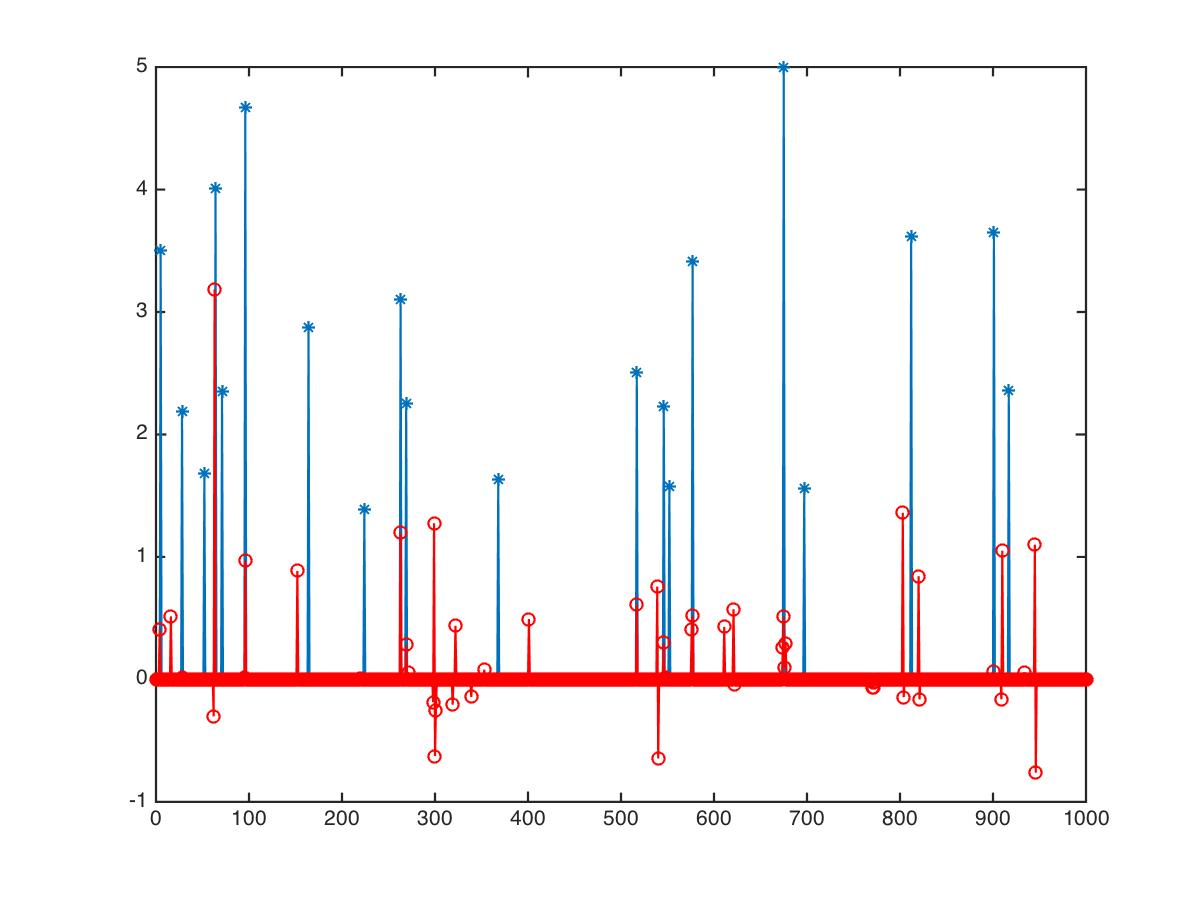
\includegraphics[width=.6\textwidth]{figures/421-betaBETA}
}
       \caption{ figure to be replaced }
\label{fig:1-reall23}
\end{figure} 


%\section*{Step 4}
~\\

1. c.f. the code directory $\rightarrow 'dataset\_generator.m'$.\\
	
\end{document}
